%!TEX root = report.tex
\chapter{Background}

\section{London Bus Network}

\par The bus network in London is one of the largest and most accessible in the world. It is carrying a staggering number of passengers, with more than 2.4 billion journeys in 2013/14, which was more than any year since 1959 \cite{tfl_annual_report_13/14}.

\par On an average day between 2005 and 2010, about 14\% of the trips made by London residents were by bus \cite{tfl_ltds}. They spent on average 14 minutes per day on these bus trips.

\par There are currently 19,345 bus stops, and 680 routes served by 8,765 buses daily in London\cite{bus_stop_locations_routes}.

\todo[inline, color=purple]{produce graph for this, number of stops, routes and buses}
% number of people that use apps to plan journey or pick the bus to take

\subsection{Bus Network Performance}

\par TfL published the following figures in the second quarter 2014/2015 buses performance data \cite{buses_performance_report}.

\par For the high frequency services, the average scheduled wait was 4.86 minutes, the average excess wait was 0.94 minutes, and the average actual wait was 5.80 minutes. While passengers could expect the buses to come within 10 minutes 83.4\% of the time, there was 15.1\% chance of waiting for 10-20 minutes, 1.3\% chance of waiting for 20-30 minutes, and 0.2\% chance of waiting for more than 30 minutes.

\par For the low frequency services, 87\% of the buses services were on time, and 11.4\% were 5-15 minutes late.

\par For the night buses, 84.5\% of the services were on time. The average excess wait was 0.68 minutes.

\todo[inline, color=purple]{produce graph here}

\par The bus arrivals might be affected by traffic congestion, staff availability, engineering problems, or mechanical breakdown \cite{buses_performance_data}.

\section{Buses Status Updates}
\par To inform passengers of the bus service disruptions or diversions, \acrshort{tfl} provides a bus status updates service online \cite{tfl_buses_status_updates}. Passengers can retrieve relevant bus service status for a given bus stop or route (Figure \ref{fig:tfl_status_update}).

\begin{figure}
\centering
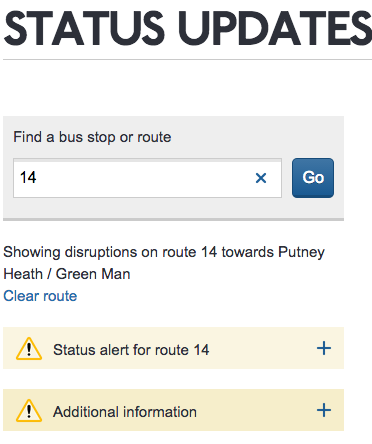
\includegraphics[width=0.5\textwidth]{figures/tfl_status_update.png}
\caption{\label{fig:tfl_status_update} Tfl Buses Status Update Service}
\end{figure}

\par The textual information include service disruptions, diversion, suspensions, and delays due to heavy traffic.

\par While this service informs passengers of current abnormal bus schedules, it requires passengers to visit the site to check for specific information, and does not provide an estimation on the travel time under the special conditions.

\par \acrshort{tfl} also publishes live status news and updates on Twitter\cite{tfl_bus_alerts_twitter}, but it is not convenient for passengers to search specific information relevant to their journeys.

\par Many current popular journey planners such as Google Maps\cite{google_maps}, Citymapper London\cite{citymapper}, and \acrshort{tfl} Journey Planner incorporate the bus delay information in the suggested journeys as a textual alert. However, these apps do not recompute the estimated journey time for passengers to make an informed decision.

\par As a result, the lack of data service on bus delay predictions and travel times estimations presents a significant barrier to bus passengers who wish to plan their bus journeys for specific appointments.

% \section{Choice of Travel Mode}
% \todo[inline]{Does the arrival time / delay affect people's choice of travel mode? What are the purposes of commute? Work, travel, leisure, appointments?}
